
%%%%%%%%%%%%%%%%%%%%%%%%%%%%%%%%%%%%%%%%%%%%%%%%%%%%%%%%%%%%%%%%%%%%%%%%%%%%%%%%
%% ************************************************************************** %%
%% *                                Settings                                * %%
%% ************************************************************************** %%
%%%%%%%%%%%%%%%%%%%%%%%%%%%%%%%%%%%%%%%%%%%%%%%%%%%%%%%%%%%%%%%%%%%%%%%%%%%%%%%%
\documentclass{tron}

\loadglsentries{gls}
\glsaddall
\addbibresource{reference}
\usepackage{xcolor}  % Coloured text etc.
% fancy note style
% STYLE NOTES : v2.0
% additional fancy boxes
\usepackage[framemethod=TikZ]{mdframed}
%\usepackage{amsthm}

% gray color indicates [OPTIONAL READING]

%%%%%%%%%%%%%%%%%%%%%%%%%%%%%%
%Note
\newenvironment{note}[3][]{%
	\ifstrempty{#1}%
	{\mdfsetup{%
	frametitle={%
	\tikz[baseline=(current bounding box.east),outer sep=0pt]
	\node[anchor=east,rectangle,fill=#2]
	{\strut Note};}}
	}%
	{\mdfsetup{%
	frametitle={%
	\tikz[baseline=(current bounding box.east),outer sep=0pt]
	\node[anchor=east,rectangle,fill=#2]
	{\strut #1};}}%
	}%
	\mdfsetup{innertopmargin=0pt,skipabove=5pt,linecolor=#2,%
		linewidth=2pt,topline=true,%
		frametitleaboveskip=\dimexpr-\ht\strutbox\relax,
		backgroundcolor={white!90!#2}}
	\begin{mdframed}[]\relax%
	\label{#3}}{\end{mdframed}
}
\Crefname{note}{Note}{notes}

\newcommand{\createnoteenv}[6]{
	\refstepcounter{#6}%
	\ifstrempty{#1}%
	{\mdfsetup{%
	frametitle={%
	\tikz[baseline=(current bounding box.east),outer sep=0pt]
	\node[anchor=east,rectangle,fill=#3]
	{\strut #4~#5};}}
	}%
	{
		\mdfsetup{%
			frametitle={%
				\tikz[baseline=(current bounding box.east),outer sep=0pt]
				\node[anchor=east,rectangle,fill=#3]
				{\strut #4~#5:~#1};
			}
		}%
	}%
	\mdfsetup{innertopmargin=0pt,skipabove=5pt,linecolor=#3,%
	linewidth=2pt,topline=true,%
	frametitleaboveskip=\dimexpr-\ht\strutbox\relax,
	backgroundcolor={white!90!#3}}
	\begin{mdframed}[]\relax%
	\label{#2}
}

%%%%%%%%%%%%%%%%%%%%%%%%%%%%%%
%Definition
\newcounter{definition}[section] \setcounter{definition}{0}
\renewcommand{\thedefinition}{\arabic{section}.\arabic{definition}}
\newenvironment{definition}[2][]{%
	\createnoteenv{#1}{#2}{blue!40}{Definition}{\thedefinition}{definition}%
}{\end{mdframed}}
\newenvironment{definition*}[2][]{%
	\createnoteenv{#1}{#2}{gray!40}{Definition}{\thedefinition}{definition}%
}{\end{mdframed}}
\Crefname{definition}{Definition}{definitions}


%%%%%%%%%%%%%%%%%%%%%%%%%%%%%%
%theoremrem
\newcounter{theorem}[section] \setcounter{theorem}{0}
\renewcommand{\thetheorem}{\arabic{section}.\arabic{theorem}}
\newenvironment{theorem}[2][]{%
	\createnoteenv{#1}{#2}{cyan!40}{Theorem}{\thetheorem}{theorem}%
}{\end{mdframed}}
\newenvironment{theorem*}[2][]{%
	\createnoteenv{#1}{#2}{gray!40}{Theorem}{\thetheorem}{theorem}%
}{\end{mdframed}}
\Crefname{theorem}{Theorem}{theorems}

%%%%%%%%%%%%%%%%%%%%%%%%%%%%%%
%Proof
\newcounter{proof}[section]\setcounter{proof}{0}
\renewcommand{\theproof}{\arabic{section}.\arabic{proof}}
\newenvironment{proof}[2][]{%
	\createnoteenv{#1}{#2}{red!20}{Proof}{\theproof}{proof}%
}{\end{mdframed}}
\newenvironment{proof*}[2][]{%
	\createnoteenv{#1}{#2}{gray!40}{Proof}{\theproof}{proof}%
}{\end{mdframed}}
\Crefname{proof}{Proof}{proofs}


%%%%%%%%%%%%%%%%%%%%%%%%%%%%%%
%Alert
\newcounter{alert}[section]\setcounter{alert}{0}
\renewcommand{\thealert}{\arabic{section}.\arabic{alert}}
\newenvironment{alert}[2][]{%
	\createnoteenv{#1}{#2}{red!80}{Alert}{\thealert}{alert}%
}{\end{mdframed}}
\newenvironment{alert*}[2][]{%
	\createnoteenv{#1}{#2}{gray!40}{Alert}{\thealert}{alert}%
}{\end{mdframed}}
\Crefname{alert}{Alert}{alerts}

%%%%%%%%%%%%%%%%%%%%%%%%%%%%%%
%Answer
\newcounter{answer}[section]\setcounter{answer}{0}
\renewcommand{\theanswer}{\arabic{section}.\arabic{answer}}
\newenvironment{answer}[2][]{%
	\createnoteenv{#1}{#2}{orange!60}{Answer}{\theanswer}{answer}%
}{\end{mdframed}}
\newenvironment{answer*}[2][]{%
	\createnoteenv{#1}{#2}{gray!40}{Answer}{\theanswer}{answer}%
}{\end{mdframed}}
\Crefname{answer}{Answer}{answers}

%%%%%%%%%%%%%%%%%%%%%%%%%%%%%%
%Remark
\newcounter{remark}[section]\setcounter{remark}{0}
\renewcommand{\theremark}{\arabic{section}.\arabic{remark}}
\newenvironment{remark}[2][]{%
	\createnoteenv{#1}{#2}{orange!40}{Remark}{\theremark}{remark}%
}{\end{mdframed}}
\newenvironment{remark*}[2][]{%
	\createnoteenv{#1}{#2}{gray!40}{Remark}{\theremark}{remark}%
}{\end{mdframed}}
\Crefname{remark}{Remark}{remarks}


%%%%%%%%%%%%%%%%%%%%%%%%%%%%%%%
%%Example
%\newcounter{example}[section]\setcounter{example}{0}
%\renewcommand{\theexample}{\arabic{section}.\arabic{example}}
%\newenvironment{example}[2][]{%
%	\createnoteenv{#1}{#2}{blue!40!cyan!20}{Example}{\theexample}{example}%
%}{\end{mdframed}}
%\newenvironment{example*}[2][]{%
%	\createnoteenv{#1}{#2}{gray!40}{Example}{\theexample}{example}%
%}{\end{mdframed}}

%%%%%%%%%%%%%%%%%%%%%%%%%%%%%%
%Algorithm
\newcounter{algo}[section]\setcounter{algo}{0}
\renewcommand{\thealgo}{\arabic{algo}.\arabic{algo}}
\newenvironment{algo}[2][]{%
	\createnoteenv{#1}{#2}{yellow!90!brown!60}{Algorithm}{\thealgo}{algo}%
}{\end{mdframed}}
\newenvironment{algo*}[2][]{%
	\createnoteenv{#1}{#2}{gray!40}{Algorithm}{\thealgo}{algo}%
}{\end{mdframed}}
\Crefname{algo}{Algorithm}{algos}

%%%%%%%%%%%%%%%%%%%%%%%%%%%%%%
% CS480 - Exercise
%\setlength{\parskip}{1cm}
%\setlength{\parindent}{1cm}

%\tikzstyle{titregris} =
%[draw=gray,fill=white, shading = exersicetitle, %
%text=gray, rectangle, rounded corners, right,minimum height=.3cm]
%\pgfdeclarehorizontalshading{exersicebackground}{100bp}
%{color(0bp)=(green!40); color(100bp)=(black!5)}
%\pgfdeclarehorizontalshading{exersicetitle}{100bp}
%{color(0bp)=(red!40);color(100bp)=(black!5)}
%\newcounter{exercise}
%\renewcommand*\theexercise{exercice \textbf{Exercice}~n\arabic{exercise}}
%\makeatletter
%\def\mdf@@exercisepoints{}%new mdframed key:
%\define@key{mdf}{exercisepoints}{%
%\def\mdf@@exercisepoints{#1}
%}
%
%\mdfdefinestyle{theoremstyle}{%
%outerlinewidth=0.01em,linecolor=black,middlelinewidth=0.5pt,%
%frametitlerule=true,roundcorner=2pt,%
%apptotikzsetting={\tikzset{mfframetitlebackground/.append style={%
%shade,left color=white, right color=blue!20}}},
%frametitlerulecolor=black,innertopmargin=1\baselineskip,%green!60,
%innerbottommargin=0.5\baselineskip,
%frametitlerulewidth=0.1pt,
%innertopmargin=0.7\topskip,skipabove={\dimexpr0.2\baselineskip+0.1\topskip\relax},
%frametitleaboveskip=1pt,
%frametitlebelowskip=1pt
%}
%\mdtheorem[style=theoremstyle]{exercise}{\textbf{Exercise}}

\newcounter{exercise}[section]\setcounter{exercise}{0}
\renewcommand{\theexercise}{\arabic{exercise}}
\newenvironment{exercise}[2][]{%
	\createnoteenv{#1}{#2}{gray!40}{Exercise}{\theexercise}{exercise}%
}{\end{mdframed}}
\newenvironment{exercise*}[2][]{%
	\createnoteenv{#1}{#2}{gray!40}{Exercise}{\theexercise}{exercise}%
}{\end{mdframed}}

\Crefname{exercise}{Exercise}{exercises}


%%%%%%%%%%%%%%%%%%%%%%%%%%%%%%
%Examples
% {

%     \section{Theorem and lemma examples with title}
%     \begin{theorem}[Pythagoras' theorem]{theorem:pythagoras}
%     In a right triangle, the square of the hypotenuse is equal to the sum of the squares of the catheti.
%     \[a^2+b^2=c^2\]
%     \end{theorem}
%     In mathematics, the Pythagorean theorem, also known as Pythagoras' theorem (see theorem \ref{theorem:pythagoras}), is a relation in Euclidean geometry among the three sides of a right triangle.
%     
%     \begin{definition}[B\'ezout's identity]{def:bezout}
%     Let $a$ and $b$ be nonzero integers and let $d$ be their greatest common divisor. Then there exist integers $x$ and $y$ such that:
%     \[ax+by=d\]
%     \end{definition}
%     This is a reference to Bezout's lemma \ref{def:bezout}
%     
%     
%     \section{Theorem and proof examples without title}
%     
%     \begin{theorem}[]{theorem:theorem1}
%     There exist two irrational numbers $x$, $y$ such that $x^y$ is rational.
%     \end{theorem}
%     
%     \begin{proof}[]{proof:proof1}
%     If $x=y=\sqrt{2}$ is an example, then we are done; otherwise $\sqrt{2}^{\sqrt{2}}$ is irrational, in which case taking $x=\sqrt{2}^{\sqrt{2}}$ and $y=\sqrt{2}$ gives us:
%     \[\bigg(\sqrt{2}^{\sqrt{2}}\bigg)^{\sqrt{2}}=\sqrt{2}^{\sqrt{2}\sqrt{2}}=\sqrt{2}^{2}=2.\]
%     \end{proof}
%
%     \begin{alert}[]{alert:alert1}
%     If $x=y=\sqrt{2}$ is an example, then we are done; otherwise $\sqrt{2}^{\sqrt{2}}$ is irrational, in which case taking $x=\sqrt{2}^{\sqrt{2}}$ and $y=\sqrt{2}$ gives us:
%     \[\bigg(\sqrt{2}^{\sqrt{2}}\bigg)^{\sqrt{2}}=\sqrt{2}^{\sqrt{2}\sqrt{2}}=\sqrt{2}^{2}=2.\]
%     \end{alert}
%     
%     \begin{remark}[]{alert:alert1}
%     If $x=y=\sqrt{2}$ is an example, then we are done; otherwise $\sqrt{2}^{\sqrt{2}}$ is irrational, in which case taking $x=\sqrt{2}^{\sqrt{2}}$ and $y=\sqrt{2}$ gives us:
%     \[\bigg(\sqrt{2}^{\sqrt{2}}\bigg)^{\sqrt{2}}=\sqrt{2}^{\sqrt{2}\sqrt{2}}=\sqrt{2}^{2}=2.\]
%     \end{remark}
%     
%     
%          \begin{exercise}[]{alert:alert1}
%     If $x=y=\sqrt{2}$ is an example, then we are done; otherwise $\sqrt{2}^{\sqrt{2}}$ is irrational, in which case taking $x=\sqrt{2}^{\sqrt{2}}$ and $y=\sqrt{2}$ gives us:
%     \[\bigg(\sqrt{2}^{\sqrt{2}}\bigg)^{\sqrt{2}}=\sqrt{2}^{\sqrt{2}\sqrt{2}}=\sqrt{2}^{2}=2.\]
%     \end{exercise}
%     
%     \begin{algo}[]{algorithm:alert1}
%     If $x=y=\sqrt{2}$ is an example, then we are done; otherwise $\sqrt{2}^{\sqrt{2}}$ is irrational, in which case taking $x=\sqrt{2}^{\sqrt{2}}$ and $y=\sqrt{2}$ gives us:
%     \[\bigg(\sqrt{2}^{\sqrt{2}}\bigg)^{\sqrt{2}}=\sqrt{2}^{\sqrt{2}\sqrt{2}}=\sqrt{2}^{2}=2.\]
%     \end{algo}
%     
%     \begin{note}[Goal]{pink}{note:goal}
%     If $x=y=\sqrt{2}$ is an example, then we are done; otherwise $\sqrt{2}^{\sqrt{2}}$ is irrational, in which case taking $x=\sqrt{2}^{\sqrt{2}}$ and $y=\sqrt{2}$ gives us:
%     \[\bigg(\sqrt{2}^{\sqrt{2}}\bigg)^{\sqrt{2}}=\sqrt{2}^{\sqrt{2}\sqrt{2}}=\sqrt{2}^{2}=2.\]
%     \end{note}

% }
%\usepackage{lipsum}                     % Dummytext
\usepackage{xargs}                      % Use more than one optional parameter in a new commands
\usepackage[colorinlistoftodos,prependcaption,textsize=normalsize]{todonotes}
%
\newcommandx{\unsure}[2][1=]{\todo[linecolor=red,backgroundcolor=red!25,bordercolor=red,#1]{#2}}
\newcommandx{\change}[2][1=]{\todo[linecolor=blue,backgroundcolor=blue!25,bordercolor=blue,#1]{#2}}
\newcommandx{\info}[2][1=]{\todo[linecolor=OliveGreen,backgroundcolor=OliveGreen!25,bordercolor=OliveGreen,#1]{#2}}
\newcommandx{\improvement}[2][1=]{\todo[linecolor=Plum,backgroundcolor=Plum!25,bordercolor=Plum,#1]{#2}}
\newcommandx{\thiswillnotshow}[2][1=]{\todo[disable,#1]{#2}}
%
\preto\printlistoftodos{
    \listoftodos[Todo List]
}

% EXAMPLES:
    % \todo[inline]{The original todo note withouth changed colours.\newline Here's another line.}
    % \lipsum[11]\unsure{Is this correct?}\unsure{I'm unsure about also!}
    % \lipsum[11]\change{Change this!}
    % \lipsum[11]\info{This can help me in chapter seven!}
    % \lipsum[11]\improvement{This really needs to be improved!\newline\newline What was I thinking?!}
    % \lipsum[11]
    % \thiswillnotshow{This is hidden since option `disable' is chosen!}
    % \improvement[inline]{The following section needs to be rewritten!}
    % \lipsum[11]
    % \newpage
    % \listoftodos[Notes]
%%%  Equation Condition
\newenvironment{eqconditions}
  {\par\vspace{\abovedisplayskip}\noindent\begin{tabular}{>{$}l<{$} @{${}={}$} l}}
  {\end{tabular}\par\vspace{\belowdisplayskip}}
\newenvironment{eqconditions*}
  {\noindent\begin{tabular}{>{$}l<{$} @{${}={}$} l}}
  {\end{tabular}}
%%% introduce 4th depth with \paragraph command
\usepackage{titlesec}
\setcounter{secnumdepth}{4}
\titleformat{\paragraph}
{\normalfont\normalsize\bfseries}{\theparagraph}{1em}{}
\titlespacing*{\paragraph}
{0pt}{3.25ex plus 1ex minus .2ex}{1.5ex plus .2ex}

%%% enumeration reference
% constraint
\newlist{constraint-list}{enumerate}{1}
\setlist[constraint-list,1]{leftmargin=*, label= \Roman*}
\creflabelformat{Constraint}{#2#1#3}
\crefname{constraint-listi}{Constraint}{position}
% criteria
\newlist{criteria-list}{enumerate}{1}
\setlist[criteria-list,1]{leftmargin=*, label= \Roman*}
\creflabelformat{Criterion}{#2#1#3}
\crefname{criteria-listi}{Criterion}{position}
% property
\newlist{property-list}{enumerate}{1}
\setlist[property-list,1]{leftmargin=*, label= \Roman*}
\creflabelformat{Property}{#2#1#3}
\crefname{property-listi}{Property}{position}
% assumption
\newlist{assumption-list}{enumerate}{1}
\setlist[assumption-list,1]{leftmargin=*, label= \Roman*}
\creflabelformat{Assumption}{#2#1#3}
\crefname{assumption-listi}{Assumption}{position}

% custom math command
\newcommand{\unit}[1]{\left[\si{#1}\right]}

% additional math packages
\usepackage{physics}
\usepackage{cancel}

% TODO Flags
\newcommand\TODO[1]{{\textcolor{red}{\textbf{#1}}}}
\newcommand\COMMENT[1]{\hl{#1}}

% Custom Format
% \usepackage{float}
% \usepackage[table]{xcolor}
% \usepackage{soul}
\usepackage{multirow}
\usepackage{caption} 
\captionsetup[table]{skip=3pt}
\captionsetup[figure]{skip=0pt}
\titlespacing*{\section}
{0pt}{10pt}{3pt}
\titlespacing*{\subsection}
{0pt}{8pt}{3pt}
\titlespacing*{\subsubsection}
{0pt}{8pt}{3pt}
%hide the highlight box
\hypersetup{
    colorlinks,
    linkcolor={black!50!black},
    citecolor={black!50!blue},
    urlcolor={black!80!black}
}%hide the highlight box

% table formatting
% \setlength{\arrayrulewidth}{1mm}
% \setlength{\tabcolsep}{18pt}
% \renewcommand{\arraystretch}{2.5}
\usepackage{array}
\newcolumntype{C}[1]{>{\centering\let\newline\\\arraybackslash\hspace{0pt}}m{#1}}

% custom math symbol
%% CS 480 %%
\newcommand{\bm}[1]{\mathbf{#1}}
%%%%%%%%%%%%
\newcommand{\RR}{\mathds{R}}
\newcommand{\Id}{\mathbb{I}}
\newcommand{\NN}{\mathds{N}}
\newcommand{\sign}{\mathop{\mathrm{sign}}}
\newcommand{\diag}{\mathop{\mathrm{diag}}}
\newcommand{\argmin}{\mathop{\mathrm{argmin}}}
\newcommand{\zero}{\mathbf{0}}
\newcommand{\one}{\mathbf{1}}
\newcommand{\av}{\mathbf{a}}
\newcommand{\bv}{\mathbf{b}}
\newcommand{\sv}{\mathbf{s}}
\newcommand{\Xv}{\mathbf{X}}
\newcommand{\Yv}{\mathbf{Y}}
\newcommand{\wv}{\mathbf{w}}
\newcommand{\xv}{\mathbf{x}}
\newcommand{\yv}{\mathbf{y}}
\newcommand{\zv}{\mathbf{z}}
\newcommand{\uv}{\mathbf{u}}
\newcommand{\rv}{\mathbf{r}}
\newcommand{\inner}[2]{\langle #1, #2 \rangle}
\newcommand{\red}[1]{{\color{red}#1}}
\newcommand{\blue}[1]{{\color{blue}#1}}
\newcommand{\magenta}[1]{{\color{magenta}#1}}


\newcommand{\ea}{{et al.}\xspace}
\newcommand{\eg}{{e.g.}\xspace}
\newcommand{\ie}{{i.e.}\xspace}
\newcommand{\iid}{{i.i.d.}\xspace}
\newcommand{\cf}{{cf.}\xspace}
\newcommand{\wrt}{{w.r.t.}\xspace}
\newcommand{\aka}{{a.k.a.}\xspace}
\newcommand{\etc}{{etc.}\xspace}
\newcommand{\sgm}{\mathsf{sgm}}
\newcommand{\Dc}{\mathcal{D}}
\newcommand{\ans}[1]{{\textcolor{orange}{\textsf{Ans}: #1}}}



% extra mod
\newcommand{\mref}[1]{\underline{\textbf{\hypersetup{linkcolor=orange}\Cref{#1}\hypersetup{linkcolor=blue}}}}
\usepackage{longtable}
\usepackage{float}
\usepackage{color, colortbl}
%%%%%%%%%%%%%%%%%%%%%%%%%%%%%%%%%%%%%%%%%%%%%%%%%%%%%%%%%%%%%%%%%%%%%%%%%%%%%%%%
% Make sure the following block contains the correct information               %
%%%%%%%%%%%%%%%%%%%%%%%%%%%%%%%%%%%%%%%%%%%%%%%%%%%%%%%%%%%%%%%%%%%%%%%%%%%%%%%%
\reporttitle{ECE 457B - Assignment 1}
% \selfstudy % comment this line if this is not a self study report 
% \employername{Employer Name}
% \employerstreetaddress{Employer Address}
% \employerlocation{City, Provice, Country}
\university{University of Waterloo}
\faculty{Faculty of Engineering}%Faculty of Engineering
\department{}%Department of Systems Design Engineering
\groupnumber{1}
\authornameA{Jianxiang (Jack) Xu}
\studentnumberA{20658861}
\reportdate{\today}
%\confidential{1} % comment this line if this is not a confidential report
%\authorstreetaddress{##}
%\authorlocation{##}
%\authorpostalcode{##}
\useheader % comment this line if no need for header
%%%%%%%%%%%%%%%%%%%%%%%%%%%%%%%%%%%%%%%%%%%%%%%%%%%%%%%%%%%%%%%%%%%%%%%%%%%%%%%%
% end of information block...                                                  %
%%%%%%%%%%%%%%%%%%%%%%%%%%%%%%%%%%%%%%%%%%%%%%%%%%%%%%%%%%%%%%%%%%%%%%%%%%%%%%%%

\begin{document}
%%%%%%%%%%%%%%%%%%%%%%%%%%%%%%%%%%%%%%%%%%%%%%%%%%%%%%%%%%%%%%%%%%%%%%%%%%%%%%%%
%% ************************************************************************** %%
%% *                               Title Page                               * %%
%% ************************************************************************** %%
%%%%%%%%%%%%%%%%%%%%%%%%%%%%%%%%%%%%%%%%%%%%%%%%%%%%%%%%%%%%%%%%%%%%%%%%%%%%%%%%
\maketitle
%%%%%%%%%%%%%%%%%%%%%%%%%%%%%%%%%%%%%%%%%%%%%%%%%%%%%%%%%%%%%%%%%%%%%%%%%%%%%%%%
%% ************************************************************************** %%
%% *                           Table of Contents                            * %%
%% ************************************************************************** %%
%%%%%%%%%%%%%%%%%%%%%%%%%%%%%%%%%%%%%%%%%%%%%%%%%%%%%%%%%%%%%%%%%%%%%%%%%%%%%%%%
\tableofcontents
%%%%%%%%%%%%%%%%%%%%%%%%%%%%%%%%%%%%%%%%%%%%%%%%%%%%%%%%%%%%%%%%%%%%%%%%%%%%%%%%
%% ************************************************************************** %%
%% *                            List of Figures                             * %%
%% ************************************************************************** %%
%%%%%%%%%%%%%%%%%%%%%%%%%%%%%%%%%%%%%%%%%%%%%%%%%%%%%%%%%%%%%%%%%%%%%%%%%%%%%%%%
% \listoffigures
%%%%%%%%%%%%%%%%%%%%%%%%%%%%%%%%%%%%%%%%%%%%%%%%%%%%%%%%%%%%%%%%%%%%%%%%%%%%%%%%
%% ************************************************************************** %%
%% *                             List of Tables                             * %%
%% ************************************************************************** %%
%%%%%%%%%%%%%%%%%%%%%%%%%%%%%%%%%%%%%%%%%%%%%%%%%%%%%%%%%%%%%%%%%%%%%%%%%%%%%%%%
% \listoftables
%%%%%%%%%%%%%%%%%%%%%%%%%%%%%%%%%%%%%%%%%%%%%%%%%%%%%%%%%%%%%%%%%%%%%%%%%%%%%%%%
%% ************************************************************************** %%
%% *                              MAIN BODY                                 * %%
%% ************************************************************************** %%
%%%%%%%%%%%%%%%%%%%%%%%%%%%%%%%%%%%%%%%%%%%%%%%%%%%%%%%%%%%%%%
\clearpage
\pagenumbering{arabic}
\setcounter{page}{1}
\setlength{\parskip}{5pt}
\newpage

%%%%%%%%%%%%%%%%%%%%%%%%%%%%%%%%%%%
%%%%% Intro.  %%%%%%
%%%%%%%%%%%%%%%%%%%%%%%%%%%%%%%%%%%

%%%%%%%%%%%%%%%%
%%%%% Ex 1 %%%%%
%%%%%%%%%%%%%%%%
\newpage
\section{Problem 1: Perceptron [Full Implementation: \Cref{code:p1}]}

%%%%%%% 1.a)
\subsection{(a): Derivation of $\Delta w_i$ (5 marks)}
{	
	\begin{align}
		\nabla_w E(w) 		& = \frac{\partial \left[ \frac12 \left( t^{(k)} - s(\sum_i w_i x_i^{(k)}) \right)^2 \right]}{\partial w}\\
		\textbf{Let } f(w) 	& = t^{(k)} - s(\sum_i w_i x_i^{(k)}) \\
							& \therefore \quad \nabla_w E(w) = \frac{\partial \left[ \frac12 \left( f(w) \right)^2 \right]}{\partial w} = f(w) \frac{\partial f(w)}{\partial w}\\
		\textbf{Let } g(w) & = \sum_i w_i x_i^{(k)} \\
							& \therefore \quad \frac{\partial f(w)}{\partial w} = \frac{\partial \left[t^{(k)} - s(\sum_i w_i x_i^{(k)})\right]}{\partial w} = \frac{\partial \left[t^{(k)} - s(g(w))\right]}{\partial w} = \frac{\partial \left[- s(g(w))\right]}{\partial w} \\
							& \because \quad s'(x) = s(x)(1 - s(x)) \text{ [Sigmoid Derivative]}\\
							& \therefore \quad \frac{\partial f(w)}{\partial w} = - \left[ s(g(w)) \right]\cdot\left[ 1 - s(g(w))\right] \cdot \frac{\partial g(w)}{\partial w}\\
							& \because \quad \frac{\partial g(w)}{\partial w} = \frac{\partial \left[  \sum_i w_i x_i^{(k)} \right]}{\partial w} =  \sum_i x_i^{(k)} \\
							& \therefore \quad \frac{\partial f(w)}{\partial w} = - \left[ s(g(w)) \right]\cdot\left[ 1 - s(g(w))\right] \cdot \sum_i x_i^{(k)}\\
		\therefore \quad \nabla_w E(w) 	&= f(w) \frac{\partial f(w)}{\partial w}\\
									   	&= \left[ t^{(k)} - s(\sum_i w_i x_i^{(k)}) \right] \cdot \left\{ - \left[ s(g(w)) \right]\cdot\left[ 1 - s(g(w))\right] \cdot \sum_i x_i^{(k)} \right\} \\
									   	&= \left[ t^{(k)} - s(\sum_i w_i x_i^{(k)}) \right] \cdot \left\{ - \left[ s(\sum_i w_i x_i^{(k)}) \right]\cdot\left[ 1 - s(\sum_i w_i x_i^{(k)})\right] \cdot \sum_i x_i^{(k)} \right\} \\
									   	&= \left[ t^{(k)} - s(\sum_i w_i x_i^{(k)}) \right] \cdot \left\{ - \left[ \frac1{1 + e^{- (\sum_i w_i x_i^{(k)})}} \right]\cdot\left[ 1 - \frac1{1 + e^{- (\sum_i w_i x_i^{(k)})}}\right] \cdot \sum_i x_i^{(k)} \right\} \\
									   	&= \left[ t^{(k)} - s(\sum_i w_i x_i^{(k)}) \right] \cdot \left\{ - \left[ \frac{e^{- (\sum_i w_i x_i^{(k)})}}{\left[1 + e^{- (\sum_i w_i x_i^{(k)})} \right]^2} \right] \cdot \sum_i x_i^{(k)} \right\} \\
		\textbf{By definitions: } s & =  s(g(w)) = s(\sum_i w_i x_i^{(k)}) = \frac1{1 + e^{- (\sum_i w_i x_i^{(k)})}}\\
		\therefore \quad \nabla_w E(w) &=  \left[ t^{(k)} - s \right] \cdot \left\{ - \left[ e^{- (\sum_i w_i x_i^{(k)})} \cdot s^2 \right] \cdot \sum_i x_i^{(k)} \right\}\\
										&= - \left( t^{(k)} - s \right)\left( s^2 \cdot e^{- (\sum_i w_i x_i^{(k)})} \right) \cdot \sum_i x_i^{(k)}	
	\end{align}

	\textbf{As a result:}
	\begin{align}
		\because \quad & \nabla_w E(w) = \sum_i (\nabla_w E(w))_i\\
		\therefore	\quad & (\nabla_w E(w))_i =  - \left( t^{(k)} - s \right)\left( s^2 \cdot e^{- (\sum_i w_i x_i^{(k)})} \right) \cdot x_i^{(k)}\\
		\therefore	\quad & \Delta w_i  = -\eta (\Delta_w E(w))_i = \eta \left( t^{(k)} - s \right)\left( s^2 \cdot e^{- (\sum_i w_i x_i^{(k)})} \right) x_i^{(k)}
	\end{align}
	
	\begin{eqn}[Final Derived Equation]{}
			\Delta w_i  = \eta \left( t^{(k)} - s \right)\left( s^2 \cdot e^{\left(- \sum_i w_i x_i^{(k)}\right)} \right) x_i^{(k)}
	\end{eqn}
	\textbf{Q.E.D.}
}

%%%%%%% 1.b) 
\newpage
\subsection{(b): Programs}
%\textbf{b) (5 marks) Write two small programs implementing the weight update rule for the perceptron and the Adaline for an arbitrary number of input (dimension of input x) and arbitrary training patterns. Initial values for the weights could be selected randomly in the interval [-1 1].}
The implementation can be seen in \Cref{code:perceptron} and \Cref{code:adaline}:

\lstinputlisting[language=python, caption=Perceptron Implementation, label=code:perceptron, firstline=19, lastline=50]{../src_code/output_scripts/p1.py}	

\lstinputlisting[language=python, caption=Adaline Implementation, label=code:adaline, firstline=53, lastline=102]{../src_code/output_scripts/p1.py}	

\vspace{-5pt}
\begin{alert}[Assumption]{}
	For the perceptron program, the assumption on binary data label is $\in \{-1, 1\}$, hence, there would be data augmentation before feeding in training dataset if there is a need. In addition, the weight vector has been padded with the bias term as $w_0$, hence, there is an prior assumption on the dataset for an increased dimension of $(1+d)$, with $d$ in terms of the data dimension.
\end{alert}

In addition, to better tune the training parameters and monitor the progress of the algorithm, their progress would also be plotted with \Cref{code:report}.
\lstinputlisting[language=python, caption=Progress Report Implementation For Perceptron and Adaline, label=code:report, firstline=104, lastline=139]{../src_code/output_scripts/p1.py}

%%%%%%% 1.c)
\newpage
\subsection{(c): Training Result}
%\textbf{c) (10 marks) We need to classify the following patterns using boundaries obtained from the perceptron and the Adaline.}
% These data points are located in 3D space and the first component x 0 of each vector is the artificial input associated with w 0 , which plays the role of the bias term ( -q ). The remaining entries of the vector are the actual location of the data point in 3D space.
%If you are able to separate these classes, provide the equation of the boundaries in the case of the perceptron and the case of the Adaline. Draw, the data points of the two classes, and the corresponding boundaries in 3D Cartesian space (remember the first entry of each vector, is not part of the coordinate of the data point in 3D). Use the value of h as 0.6
\subsubsection{Perceptron Training Result}
	Training Progress (where we can see the convergence of the algorithm):
	
	{	
			\centering
			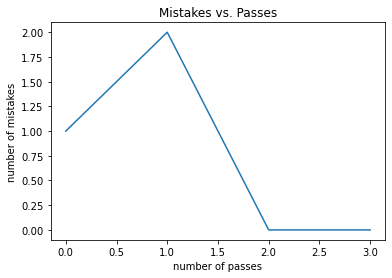
\includegraphics[height=180px]{../src_code/fig/p1/p1_perceptron_progress}
	      	\captionof{figure}{Perceptron Training Progress  \label{fig:q1:c:perceptron:progress}}
	}	
	
	\begin{eqn}[Hyperplane Equation]{}
		1.818 x + -2.540 y + -0.132 z = 1.634
	\end{eqn}
	
	The resultant hyperplane:
	
	{	
			\centering
			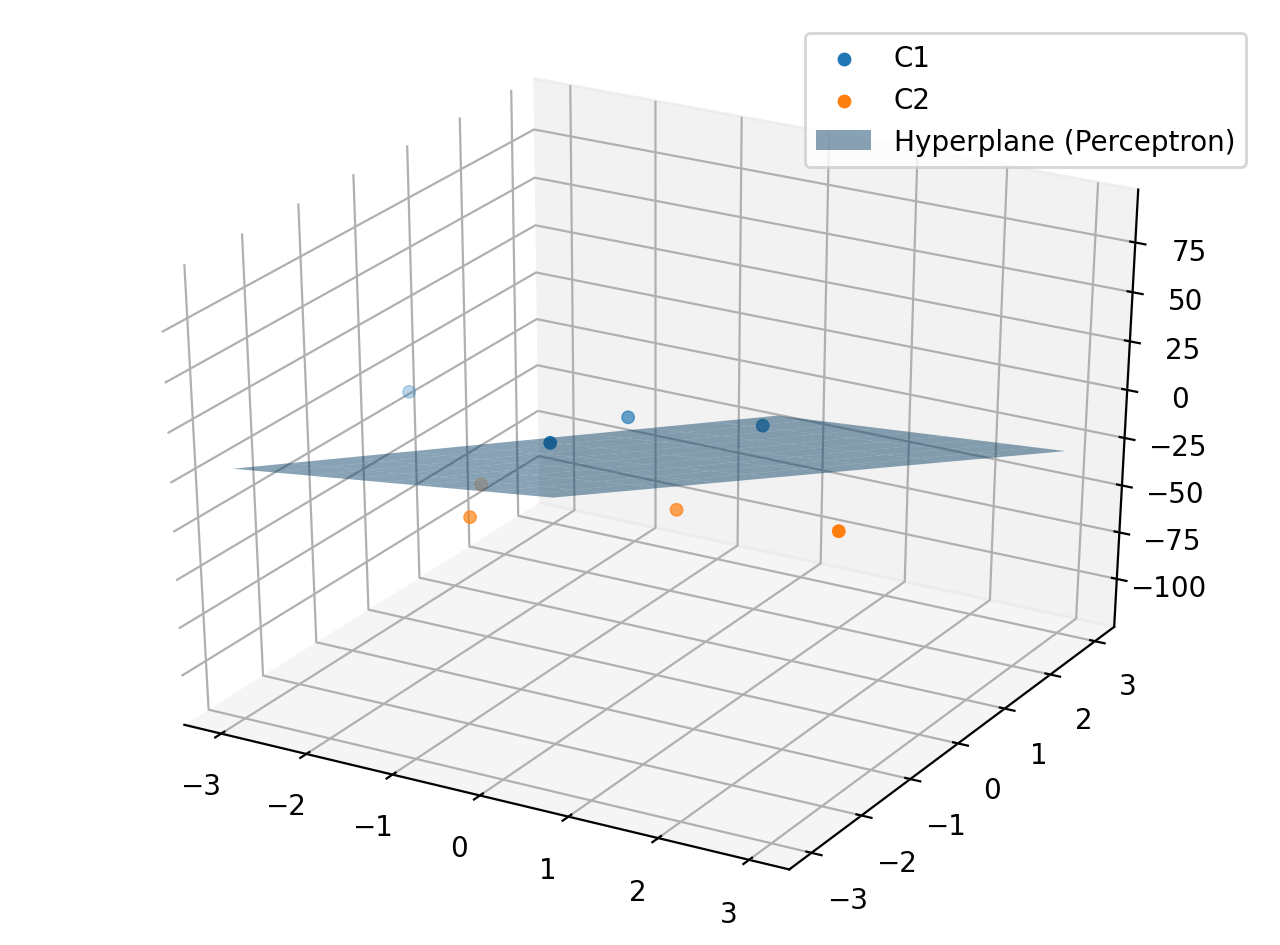
\includegraphics[height=250px]{../src_code/fig/p1/p1_plot3d_perceptron}
	      	\captionof{figure}{Perceptron Hyperplanes Result in 3D  \label{fig:q1:c:perceptron:result}}
	}	
	
	\begin{alert}[Label Modification Needed]{}
		The given class label $\in \{0,1\}$ may not lead to a convergence of the perceptron, and the label shall be transformed into $\in\{-1,1\}$. Here is showing the modified result.	
		
		$TRAIN_Y = [-1,-1,-1,-1,1,1,1,1]$
	\end{alert}


\clearpage
\subsubsection{Adaline Training Result}
	Training Progress (where we can see the convergence of the algorithm):
	
	{	
			\centering
			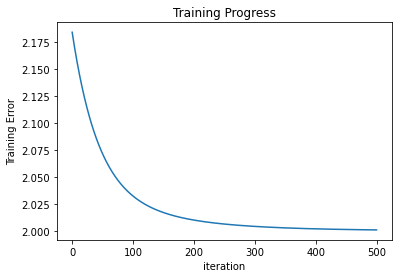
\includegraphics[height=180px]{../src_code/fig/p1/p1_adaline_training_progress_}
	      	\captionof{figure}{Adaline Training Progress  \label{fig:q1:c:adaline:progress}}
	}	
	
	\begin{eqn}[Hyperplane Equation]{}
		0.143 x + -0.757 y + 0.095 z = 0.740
	\end{eqn}
	
	The resultant hyperplane:
	
	\begin{figure}[H]
		\centering
		\subfloat[Nominal View Angle]{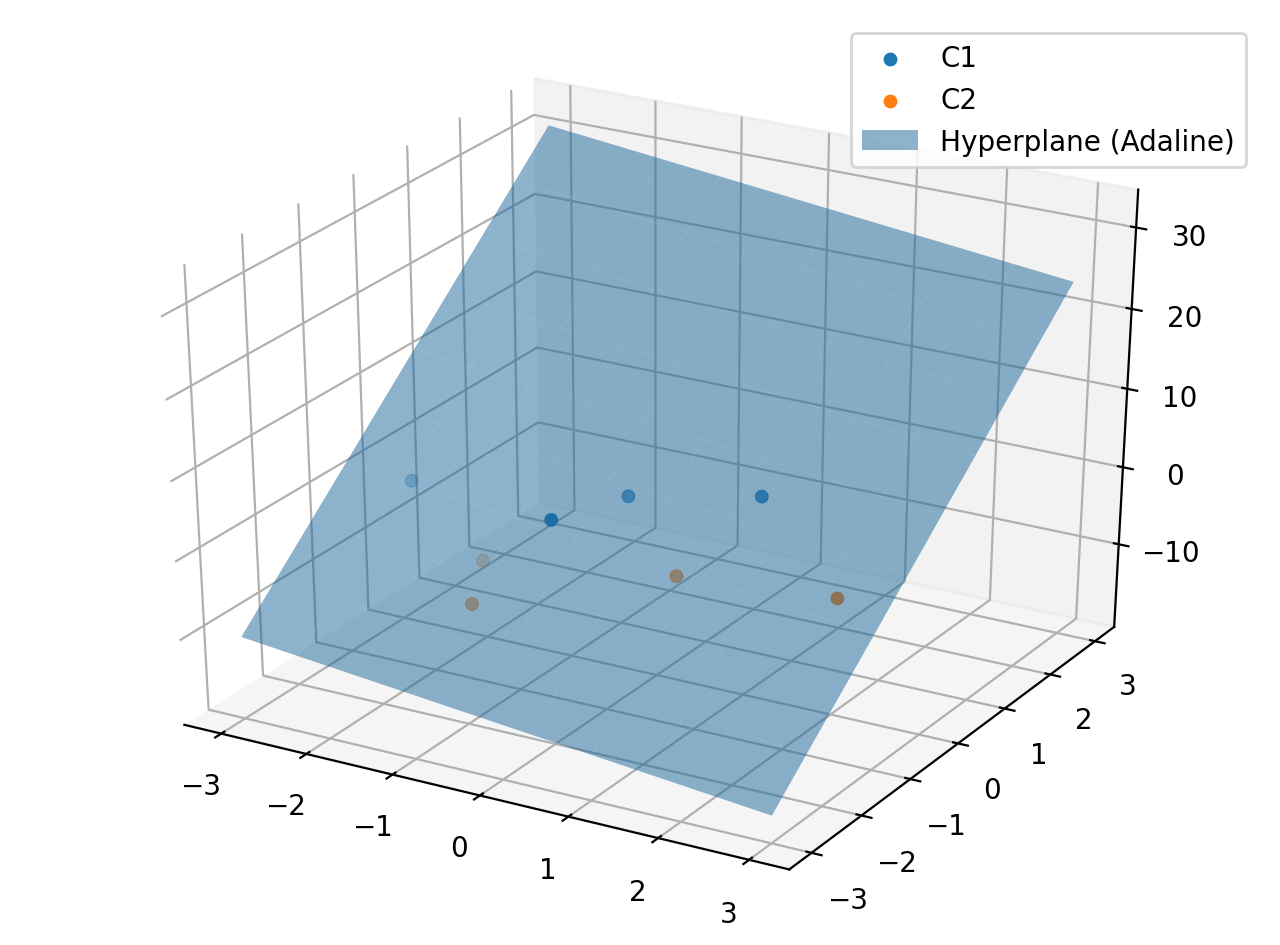
\includegraphics[height=190px]{../src_code/fig/p1/p1_plot3d_Adaline}}
		\subfloat[Modified View Angle]{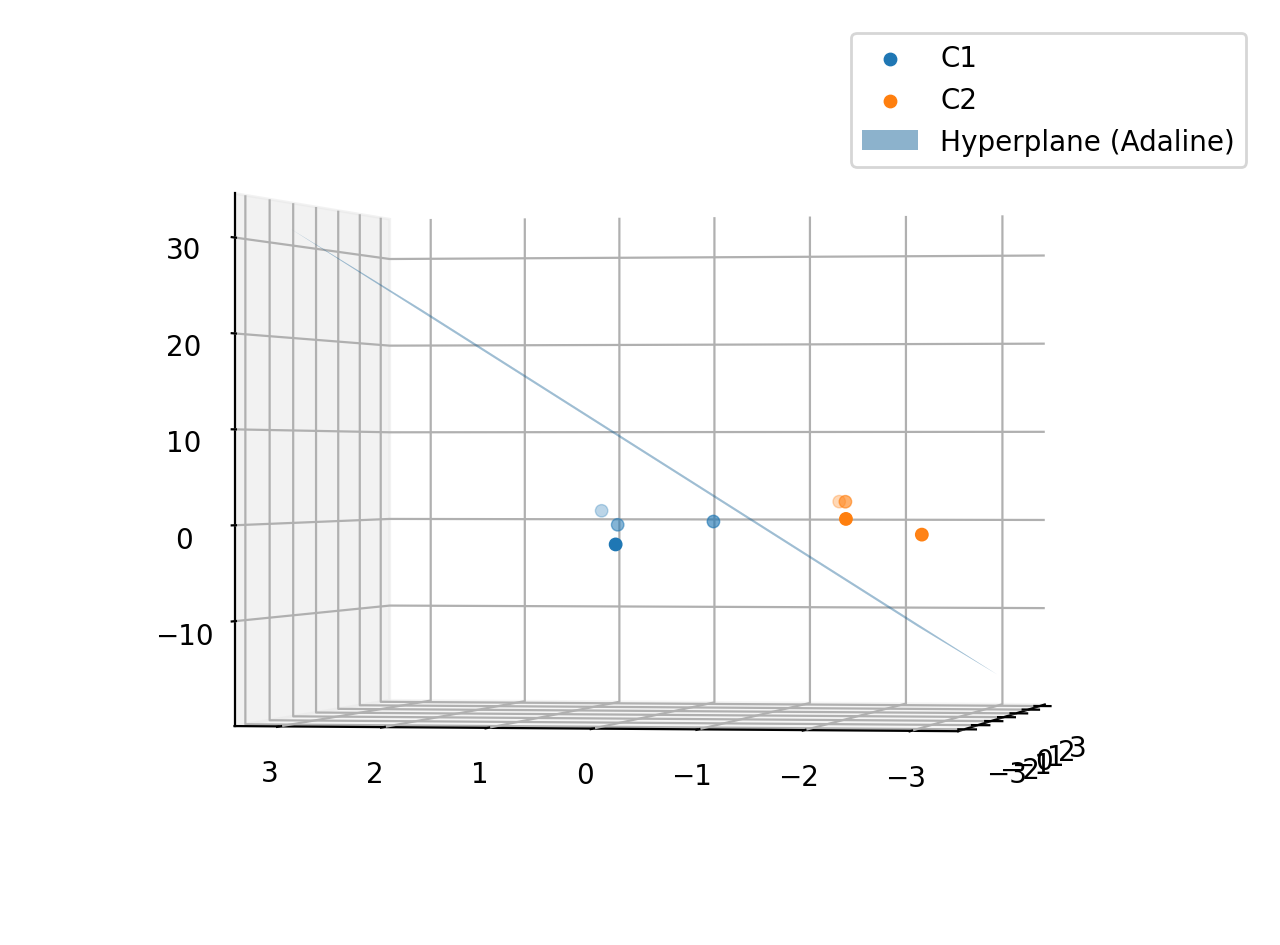
\includegraphics[height=190px]{../src_code/fig/p1/p1_plot3d_Adaline(div)}}	
		\caption{Adaline Hyperplanes Result in 3D  \label{fig:q1:c:adaline:result}}
	\end{figure}

	\begin{remark}[Label Modification Not Required]{}
		The given class label $\in \{0,1\}$ would also lead to a convergence of the adaline, but for a fair comparison, the label here shall be $\in\{-1,1\}$. Here is showing the modified result.	
		
		$TRAIN_Y = [-1,-1,-1,-1,1,1,1,1]$
	\end{remark}



%%%%%%% 1.d)
\newpage
\subsection{(d) Test Data}
%\textbf{d) (2 marks) We need to place a new data point belonging to “C1” in the location x5 =[-1.4,- 1.5, 2]. Is the classifier boundary still valid (for both perceptron and Adaline)}
Since I define "C1" as -1 label for computation optimization and efficiency.

Let's redefine the testing data as follow:
\begin{lstlisting}[language=python, style=mystyle]
	y_test = -1
	x_test = [-1, -1.3, -1.5, 2]
\end{lstlisting}

\vspace{-20pt}
Hence, as long as the dot product with the plane norm vector agrees with the label, it would indicate the plane is a valid plane for the test data point, with ($y \, (\xv \cdot \wv) > 0$):

\begin{lstlisting}[language=python, style=mystyle]
	is_perceptron = (y_test * (np.dot(x_test, w1))) > 0
	is_adaline = (y_test * (np.dot(x_test, w2))) > 0
\end{lstlisting}

\vspace{-20pt}
With result:
\begin{lstlisting}[language=python, style=mystyle:output]
	[ Valid Plane ] Perceptron: True | Adaline: False
\end{lstlisting}

\vspace{-20pt}
Hence, the perceptron plane is good enough for the test point, whereas the hyperplane is not good for the test point. This can also be observed in \Cref{fig:q1:d:result} below:

\begin{figure}[H]
	\centering
	\subfloat[Training Dataset]{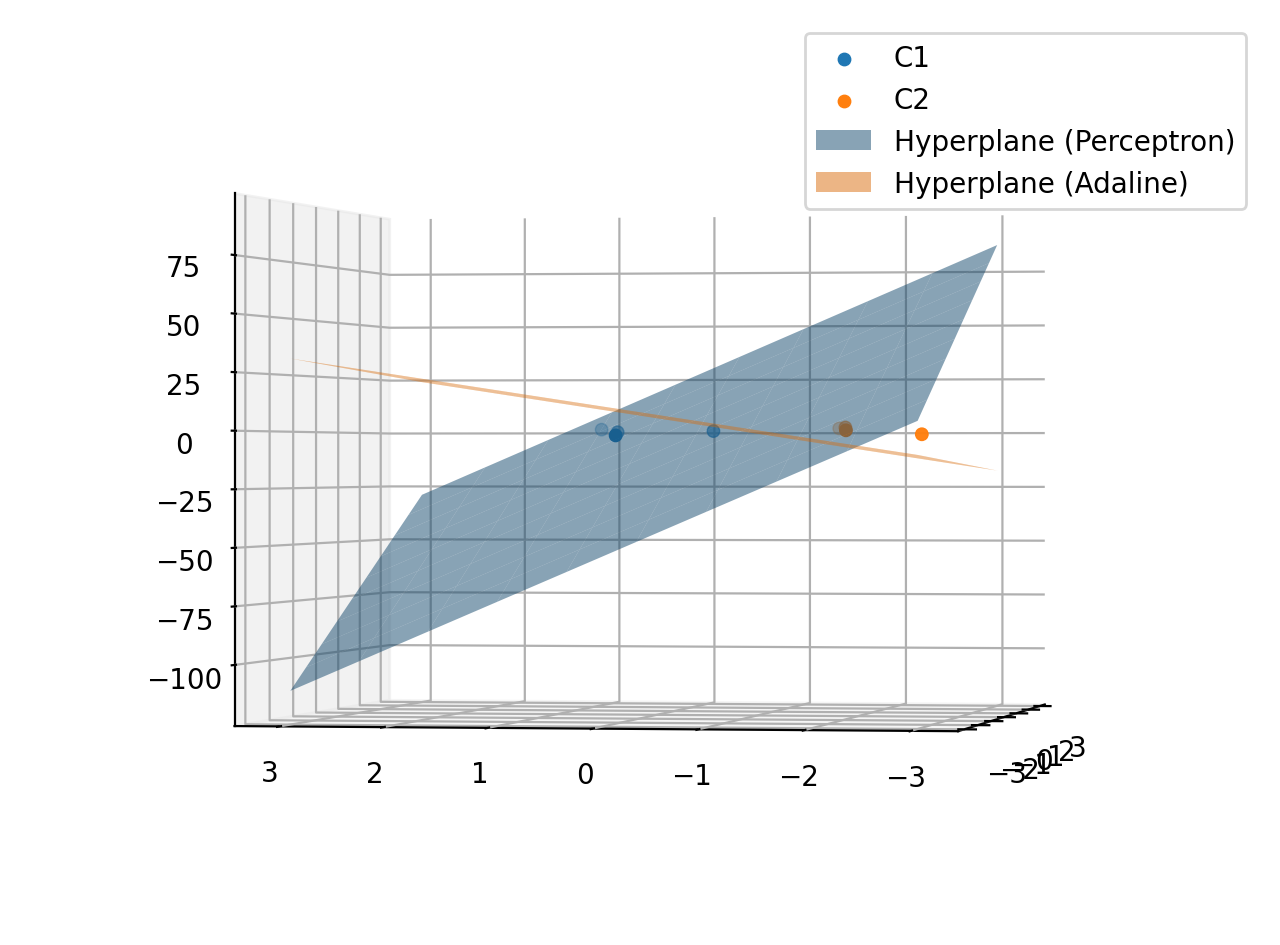
\includegraphics[height=190px]{../src_code/fig/p1/p1_plot3d_both}}
	\subfloat[Test Dataset]{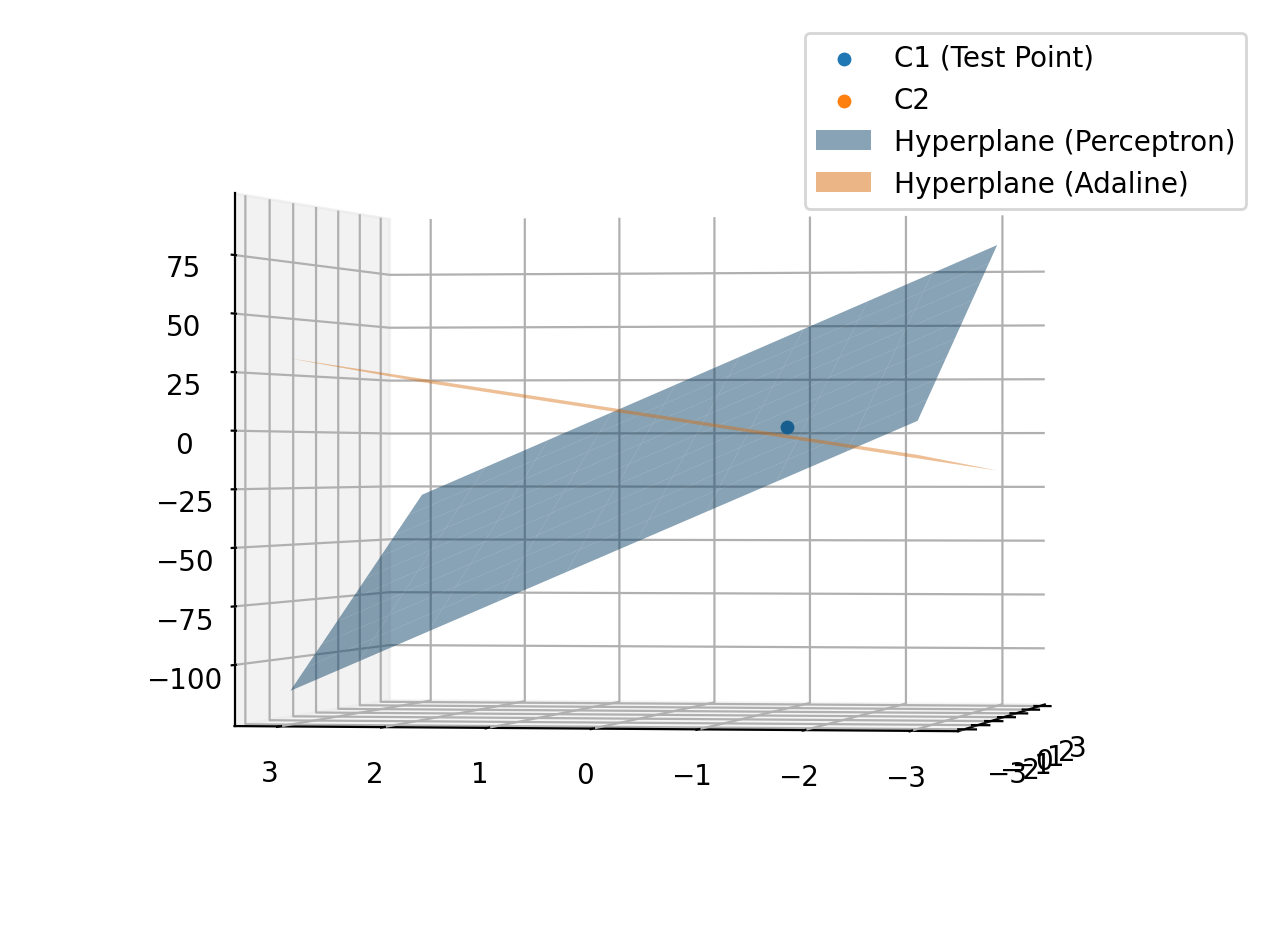
\includegraphics[height=190px]{../src_code/fig/p1/p1_plot3d_test_point}}
	\caption{Hyperplanes visualization with training dataset [Left] and test point [Right] in 3D  \label{fig:q1:d:result}}
\end{figure}

%%%%%%% 1.e)
\newpage
\subsection{(e) Why Adaline has better capabilities than perceptron in terms of learning rule}
%\textbf{e) (3 marks) State, why an Adaline structure with LMS learning algorithm has better capabilities than the perceptron Hebbian learning rule.}

They are different from the loss function, one with LMS and one with Hebbian learning rule. The LMS learning rule is a continuous and progressive learning step, whereas Hebbian learning rule is rather more discrete.
%https://www.quora.com/What-is-the-difference-between-a-Perceptron-Adaline-and-neural-network-model

Specifically, the iterations of Adaline networks do not stop at arbitrary hyperplane, instead, it converges by reducing the least mean square error.
%https://www.softwaretestinghelp.com/neural-network-learning-rules/

Whereas, the perceptron may stop with an arbitrary hyperplane depending on the order of the sampled point, whereas adaline will result an optimal and deterministic hyperplane, where its margin is the best (closest) possible geometrical plane. Since adaline utilizes the gradient decent with mean squared error, it will result a hyperplane that is close to each cluster of the dataset. In comparison, the perceptron would result an arbitrary margin with an arbitrary hyperplane, may result a non-ideal hyperplane, leading to a bias to a specific class (more close to one class).

Lastly, the perceptron requires the label to be $\in {-1, 1}$ with opposite sign, whereas, the adaline does not care much about the label sign, as long as the label is different.


%%%%%%%%%%%%%%%%
%%%%% Ex 2 %%%%%
%%%%%%%%%%%%%%%%
\newpage
\section{Problem 2: Madaline [Full Implementation: \Cref{code:p2}]}
The madaline structure would be consist of 3 fixed weights and bias:
\lstinputlisting[language=python, caption=Madaline Weights, label=code:p2, firstline=10, lastline=13]{../src_code/p2.py}	

As \Cref{fig:q2:madaline} shown, the hyperplanes with prescribed weight is able to separate the two output class (1 and -1):
\begin{figure}[H]
	\centering
	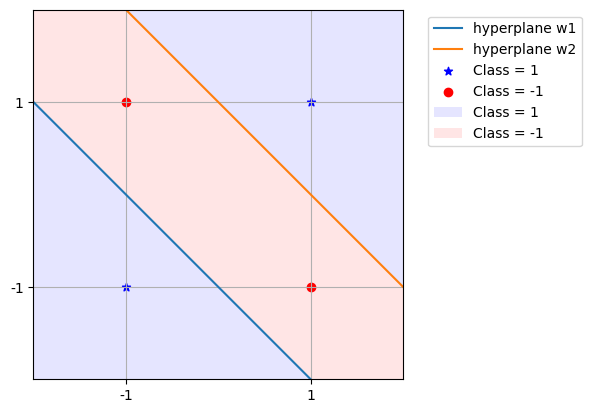
\includegraphics[height=190px]{../src_code/fig/madaline}
	\caption{Hyperplanes visualization for Madaline XNOR gate in 2D \label{fig:q2:madaline}}
\end{figure}

%%%%%%%%%%%%%%%%
%%%%% Ex 3 %%%%%
%%%%%%%%%%%%%%%%
\newpage
\section{Problem 3: BPL [Full Implementation: \Cref{code:p3}]}
\subsection{(a) Hyperparameter Tuning}
For the dataset, the program would generate an arbitrary large enough (\verb|MAX_DATA_SIZE|=500) dataset randomly in a uniform distribution. The data is then split into two portions: training data and testing data. In every combination, it will downsample the training data to a prescribed need by $i$ consistently. In every trial, it will shuffle such data to randomize the order. Within the 10-fold operation, it will split the training data into 10 pieces, and one piece would be used as validation in each iteration of the k-fold operation.

As suggested in the assignment, 16 combinations of nodes and data points have been evaluated through 5 times of the 10-fold cross validation. The best out of 5 of the averaged loss from 10-fold evaluation has been recorded for each model. The max hard stop epochs were set to 1000 iterations with early stopping condition based on validation error. The resulted matrix of validation error and training error are tabulated in \Cref{table:16tests:1} and \Cref{table:16tests:2} and graphed in \Cref{fig:p3:matrix-score:1} and \Cref{fig:p3:matrix-score:2} respectively.

\begin{table}[H]
	\centering
	\begin{tabular}{ |p{1.5cm}||p{1.5cm}|p{1.5cm}|p{1.5cm}|p{1.5cm}||p{1.5cm}|p{1.5cm}|p{1.5cm}|p{1.5cm}|  }
	 \hline
	 	& \multicolumn{4}{|c|}{Lowest Average k-Fold Training Error} & \multicolumn{4}{|c|}{Lowest Average k-Fold Validation Error} \\
	 \hline
	   	& j=2 & j=10 & j=40 & j=100 & j=2 & j=10 & j=40 & j=100\\
	 \hline
	 \hline
	i=10  & 0.04101 & 0.04728 & 0.00614 & 0.00209 & 0.00637 & 0.00940 & 0.00151 & 0.00035 \\
	\hline
	i=40  & 0.04729 & 0.04643 & 0.03344 & 0.02613 & 0.04572 & 0.05555 & 0.01800 & 0.01259 \\
	\hline
	i=80  & 0.04453 & 0.04385 & 0.03457 & 0.01004 & 0.04141 & 0.01372 & 0.01871 & \cellcolor{red!20!white} 0.00102 \\
	\hline
	i=200 & 0.05555 & 0.04532 & 0.02384 & 0.00768 & 0.03471 & 0.03724 & 0.02599 & 0.00791 \\
	\hline
	 \hline
	\end{tabular}
	\caption{Lowest average k-fold training and validation errors for $f_1(x)$}
	\label{table:16tests:1}
\end{table}

\begin{figure}[H]
	\centering
	\subfloat[Best Training Error]{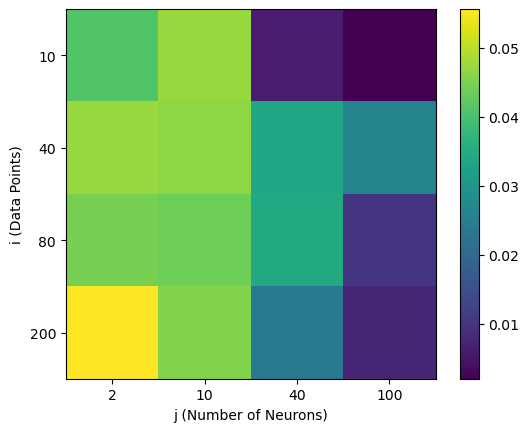
\includegraphics[height=190px]{../src_code/fig/p3/F1/matrix_lowest_training_error}}
	\subfloat[Best Validation Error]{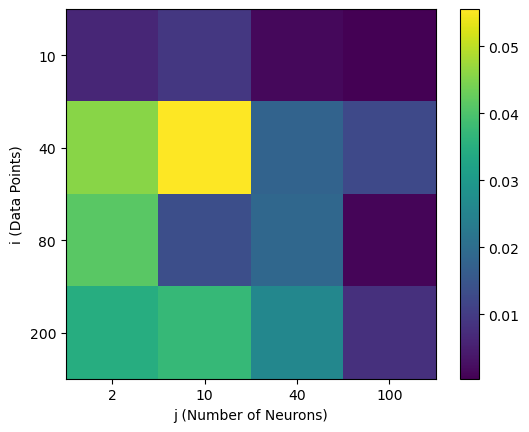
\includegraphics[height=190px]{../src_code/fig/p3/F1/matrix_lowest_validation_error}}
	\caption{Visualized lowest average k-fold errors for $f_1(x)$ \label{fig:p3:matrix-score:1}}
\end{figure}

\begin{table}[H]
	\centering
	\begin{tabular}{ |p{1.5cm}||p{1.5cm}|p{1.5cm}|p{1.5cm}|p{1.5cm}||p{1.5cm}|p{1.5cm}|p{1.5cm}|p{1.5cm}|  }
	 \hline
	 	& \multicolumn{4}{|c|}{Lowest Average k-Fold Training Error} & \multicolumn{4}{|c|}{Lowest Average k-Fold Validation Error} \\
	 \hline
	   	& j=2 & j=10 & j=40 & j=100 & j=2 & j=10 & j=40 & j=100\\
	 \hline
i=10 & 0.02760 & 0.03464 & 0.02003 & 0.00742 & 0.00169 & 0.00029 & 0.00544 & 0.00015 \\ \hline
i=40 & 0.02215 & 0.02436 & 0.01346 & 0.00432 & 0.00839 & 0.01126 & \cellcolor{red!20!white} 0.00232 & 0.00930 \\ \hline
i=80 & 0.02652 & 0.02221 & 0.01397 & 0.00634 & 0.00829 & 0.01284 & 0.00376 & 0.00549 \\ \hline
i=200& 0.02898 & 0.01951 & 0.00642 & 0.00629 & 0.02190 & 0.02035 & 0.00737 & 0.00580 \\ \hline
	\end{tabular}
	\caption{Lowest average k-fold training and validation errors for $f_2(x)$}
	\label{table:16tests:2}
\end{table}

\begin{figure}[H]
	\centering
	\subfloat[Best Training Error]{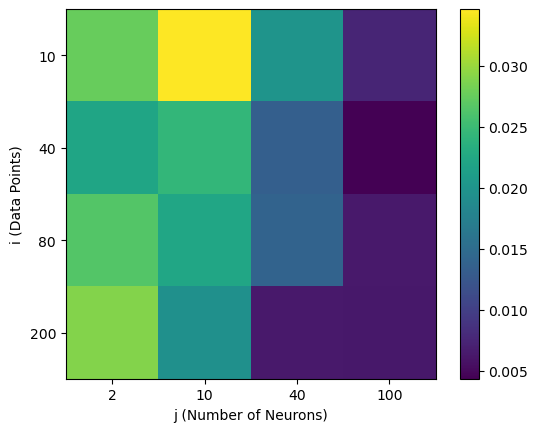
\includegraphics[height=190px]{../src_code/fig/p3/F2/matrix_lowest_training_error}}
	\subfloat[Best Validation Error]{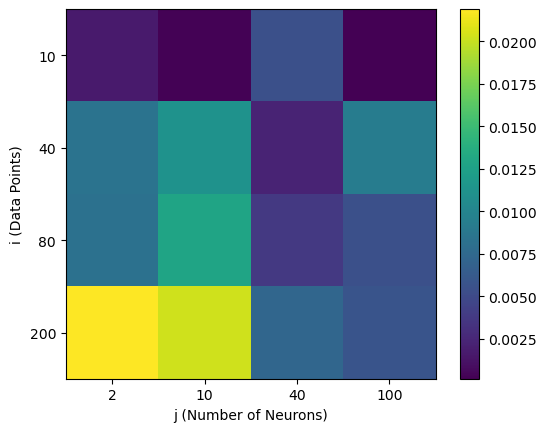
\includegraphics[height=190px]{../src_code/fig/p3/F2/matrix_lowest_validation_error}}
	\caption{Visualized lowest average k-fold errors for $f_2(x)$ \label{fig:p3:matrix-score:2}}
\end{figure}



%== Matrix lowest_training_error ===
%[[0.02394385 0.01159773 0.01121249 0.00176007]
% [0.01798267 0.02005895 0.01267773 0.00490225]
% [0.02802143 0.01936286 0.0143317  0.00347644]
% [0.02720663 0.01789071 0.00530574 0.00477603]]
%fig/p3_backup/F2/matrix_lowest_training_error.png
%== Matrix lowest_validation_error ===
%[[0.01566413 0.00105253 0.00572144 0.00013595]
% [0.02659742 0.00109245 0.00834214 0.00990521]
% [0.0076982  0.01809715 0.01161161 0.00224508]
% [0.02791829 0.01529613 0.0104063  0.00423795]]


%\newpage
\clearpage
\subsection{(b \& c) Observations and Best Fitting Results \label{sec:p2:observation}}
Based on the minimum validation error, it concludes the lowest error model is 10 data points and 100 neurons for both $f_1(x)$ and $f_2(x)$. However, this assumption quite limited, since the dataset is too small to conclude the validation. As we may see the training error is actually significantly larger than the validation error, which leads to an under-fitting model (as \Cref{fig:p3:2:underfit} suggested as what we have expected). Ideally, we expect the validation error of a good fit model is higher than training error. Hence, we may need a better model and more generalized model that has best overall errors, where the validation error does not deviate much from the training error. 

\begin{figure}[H]
	\centering
	\subfloat[Underfitting model of $f_1(x)$ \label{fig:p3:2:underfit:1}]{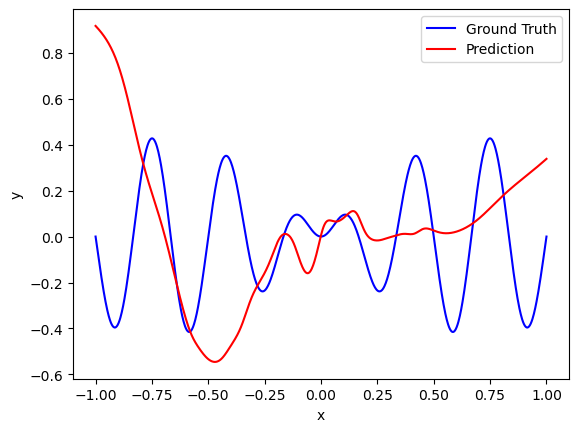
\includegraphics[height=180px]{../src_code/fig/p3/F1/final_fit_Best[Overall]}}
	\subfloat[Underfitting model of $f_2(x)$ \label{fig:p3:2:underfit:2}]{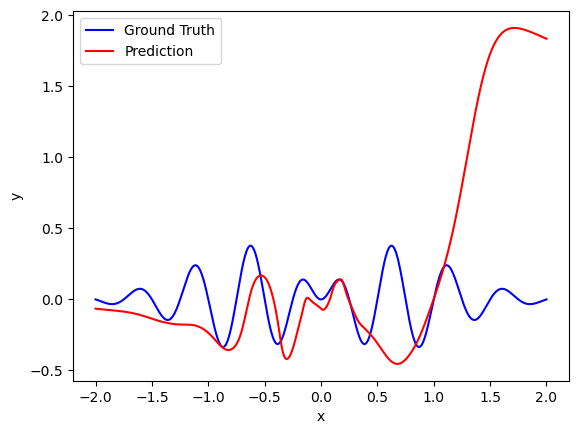
\includegraphics[height=180px]{../src_code/fig/p3/F2/final_fit_Best[Overall]}}
	\caption{Underfitting models\label{fig:p3:2:underfit}}
\end{figure}

Recall from the lecture contents, as model complexity increases (with higher $j$), it would be overfitting if the validation error also increases. The model right before such increase would be a good model. If we keep complexity unchanged, and if we observe there is an increase in validation error as the data size increases (with higher $i$), the model would be also overfitting. Hence, the one before such overfitting model would be a good model in that column. In addition, with consideration on the deviation between the training and validation error, a good model should exhibits all three characteristics.

Hence, we may conclude a good model for $f_1(x)$ based on loss matrices in \Cref{table:16tests:1} and \Cref{fig:p3:matrix-score:1} would be $(i=80, j=100)$, while a good model for $f_2(x)$ based on \Cref{table:16tests:2} and \Cref{fig:p3:matrix-score:2} would be $(i=40, j=40)$. 


As observed from \Cref{fig:p3:2:fit:1} and \Cref{fig:p3:2:fit:2} below, we can see these models are good model, that is neither overfitting nor underfitting the original function. They are much more generalized.

\begin{figure}[H]
	\centering
	\subfloat[Test Data Fitting \label{fig:p3:2:fit:1:tD}]{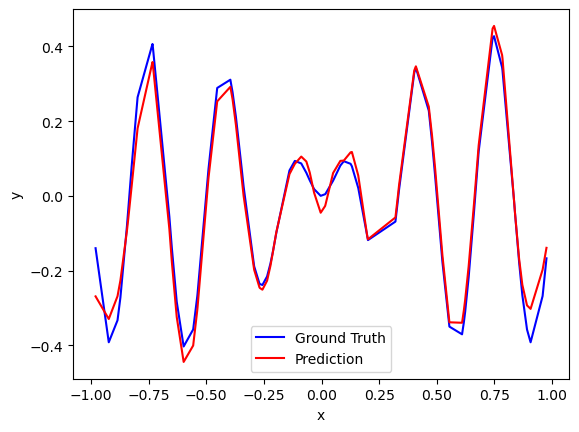
\includegraphics[height=180px]{../src_code/fig/p3/F1/final_fit_Best[Test Data]i=80-j=100}}
	\subfloat[Overall Fitting \label{fig:p3:2:fit:1:oa}]{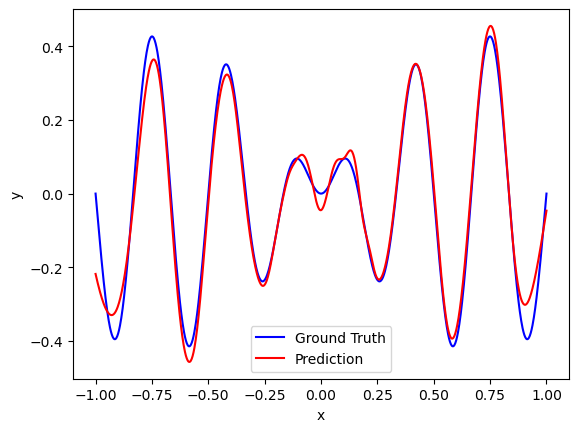
\includegraphics[height=180px]{../src_code/fig/p3/F1/final_fit_Best[Overall]i=80-j=100}}
	\caption{Final fitting of a good model $f_1(x)$ with $(i=80, j=100)$\label{fig:p3:2:fit:1}}
\end{figure}

\begin{figure}[H]
	\centering
	\subfloat[Test Data Fitting \label{fig:p3:2:fit:2:tD}]{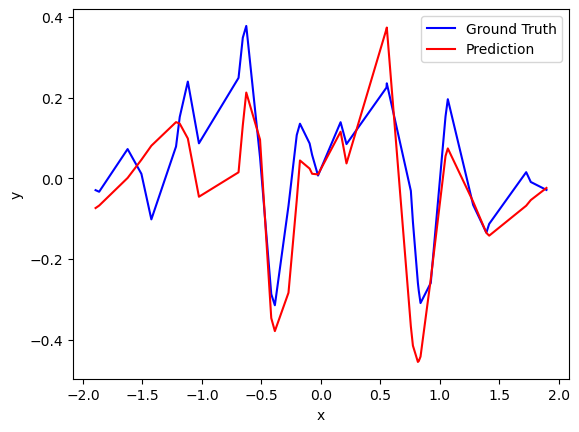
\includegraphics[height=180px]{../src_code/fig/p3/F2/final_fit_Best[Test Data]i=40-j=40}}
	\subfloat[Overall Fitting \label{fig:p3:2:fit:2:oa}]{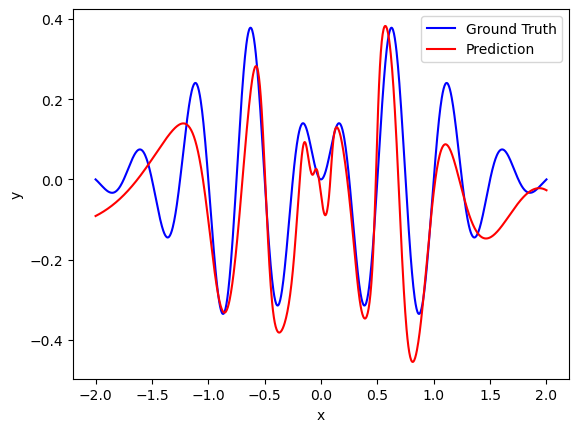
\includegraphics[height=180px]{../src_code/fig/p3/F2/final_fit_Best[Overall]i=40-j=40}}
	\caption{Final fitting of a good model $f_2(x)$ with $(i=40, j=40)$\label{fig:p3:2:fit:2}}
\end{figure}


So, what if we choose the model that uses more data points? 

As matrix suggested, we may expect an overfitting behaviour for both $f_1(x)$ and $f_2(x)$, as shown in both \Cref{fig:p3:2:fit:1:over} and \Cref{fig:p3:2:fit:2:over} for an increased dataset with $(i=200, j=100)$ and $(i=80, j=40)$ respectively.
\begin{figure}[H]
	\centering
	\subfloat[Test Data Fitting \label{fig:p3:2:fit:1:tD:over}]{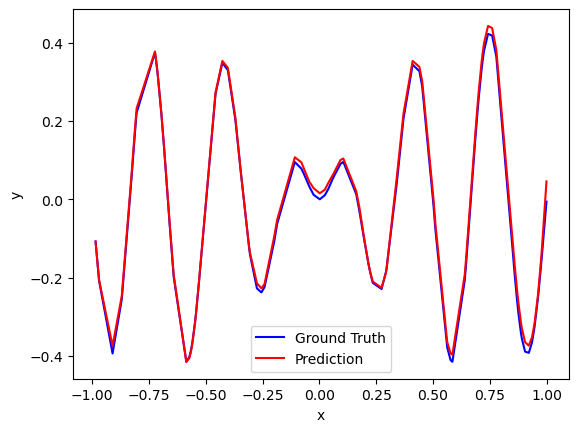
\includegraphics[height=180px]{../src_code/fig/p3/F1/final_fit_Best[Test Data]i=200-j=100}}
	\subfloat[Overall Fitting \label{fig:p3:2:fit:1:oa:over}]{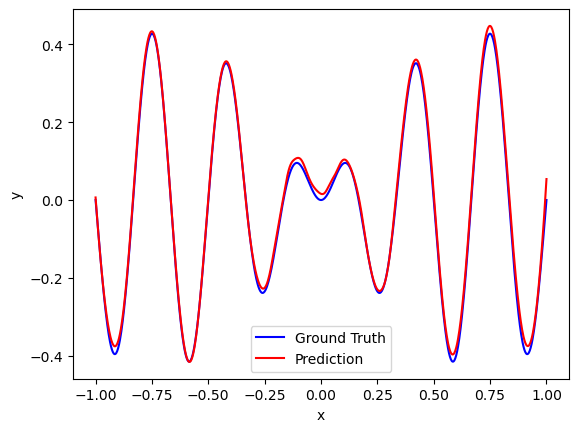
\includegraphics[height=180px]{../src_code/fig/p3/F1/final_fit_Best[Overall]i=200-j=100}}
	\caption{Overfitting model $f_1(x)$ with an increased population with $(i=200, j=100)$\label{fig:p3:2:fit:1:over}}
\end{figure}

\begin{figure}[H]
	\centering
	\subfloat[Test Data Fitting \label{fig:p3:2:fit:2:tD:over}]{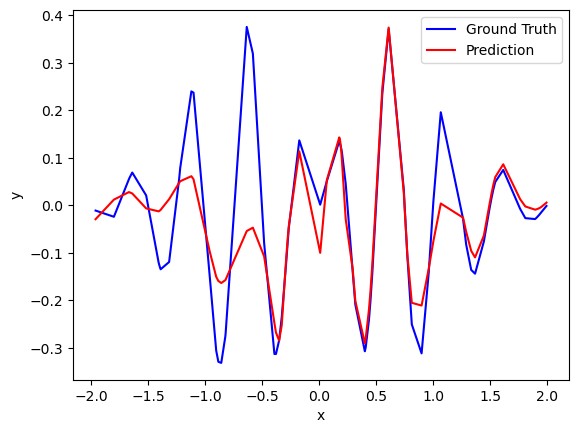
\includegraphics[height=180px]{../src_code/fig/p3/F2/final_fit_Best[Test Data]i=80-j=40}}
	\subfloat[Overall Fitting \label{fig:p3:2:fit:2:oa:over}]{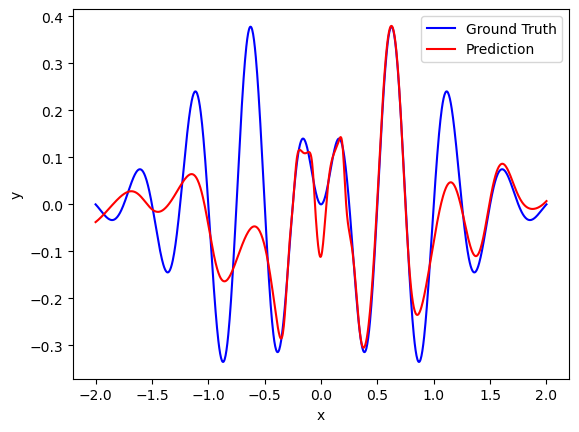
\includegraphics[height=180px]{../src_code/fig/p3/F2/final_fit_Best[Overall]i=80-j=40}}
	\caption{Overfitting model $f_2(x)$ with an increased population with $(i=80, j=40)$\label{fig:p3:2:fit:2:over}}
\end{figure}

For $f_2(x)$, we may also try to increase the model complexity, we may also observe a regional over-fitting behaviour, which ruins the overall fitting as both hyperparameter matrices (\Cref{fig:p3:matrix-score:2}) and \Cref{fig:p3:2:fit:2:over:comp} below suggested.

\begin{figure}[H]
	\centering
	\subfloat[Test Data Fitting \label{fig:p3:2:fit:2:tD:over:comp}]{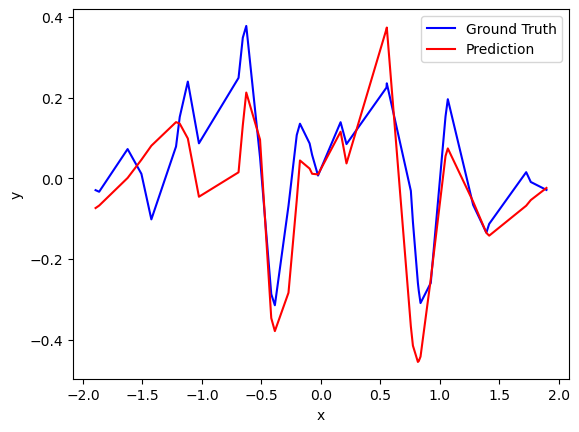
\includegraphics[height=180px]{../src_code/fig/p3/F2/final_fit_Best[Test Data]i=40-j=40}}
	\subfloat[Overall Fitting \label{fig:p3:2:fit:2:oa:over:comp}]{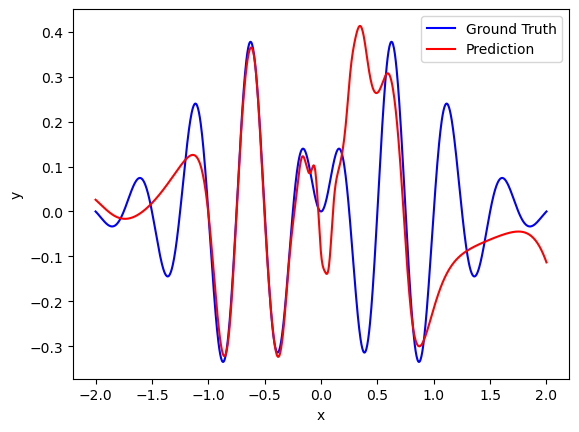
\includegraphics[height=180px]{../src_code/fig/p3/F2/final_fit_Best[Overall]i=40-j=100}}
	\caption{Overfitting model $f_2(x)$ with an increased complexity with $(i=40, j=100)$\label{fig:p3:2:fit:2:over:comp}}
\end{figure}

\subsection{(c*) Further Conclusion}
In light of lecture materials, as we observed in this experiment as discussed in \Cref{sec:p2:observation}, a good model would have a good balance of variance and bias, where it can perform well in both training and test data. Overfitting often happens when the model is too complex for the given problem or excessive amount of training dataset. In addition, excessive amount of training would also lead to an overfitting of the model, which is handled by the early stopping callbacks in our case. And k-fold validation methods indeed help us to find a suitable good model based on the error matrices.


%%%%%%%%%%%%%%%%
%%%%% Ex 4 %%%%%
%%%%%%%%%%%%%%%%
\newpage
\section{Problem 4: Neural Network Classifier [Full Implementation: \Cref{code:p4}]}
\subsection{MLP Classifier Training Result}
To train the model, we shall first normalize the given dataset. 75\% of dataset are used for training and 25\% are used to evaluate the trained model. The best performed model with highest possible testing score would be used to predict the dataset for \Cref{sec:4:2} later.

In addition, the label of the dataset is augmented into binary terms, with index of the bit as the label. For instance, label 3 would be represented by an array of $[0,0,1]$. We uses \verb|`softmax'| to make elements of output vector in range(0,1) and sum up to 1, so that the output vector is a class probability identifier. The element with highest probability shall be the class of the dataset.

To find best possible classification model, we augmented various combinations of hidden layers and nodes as stated below, with an arbitrary max-epoch as hard stop (early-termination):

\lstinputlisting[language=python, caption=Testing Models, label=code:p4, firstline=221, lastline=277]{../src_code/p4.py}

The performance results are tabulated below:
%\begin{table}
%	\centering
	\begin{longtable}{p{0.5cm} p{1.2cm} p{1.2cm} p{6cm} p{6cm}} \hline
		%% Header
		Model & Train Accuracy & Test Accuracy & Training Accuracy Progress & Training Loss Progress
		\\ \hline
		%% Content
		t1 & 98.50\% & 97.78\% & \raisebox{-125px}{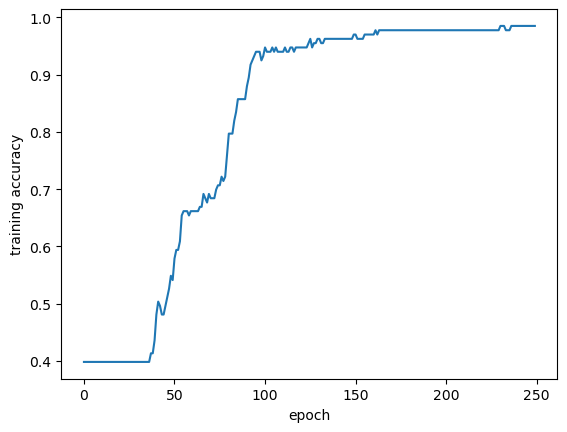
\includegraphics[height=130px]{../src_code/fig/p4/train_accu_t1}} & \raisebox{-125px}{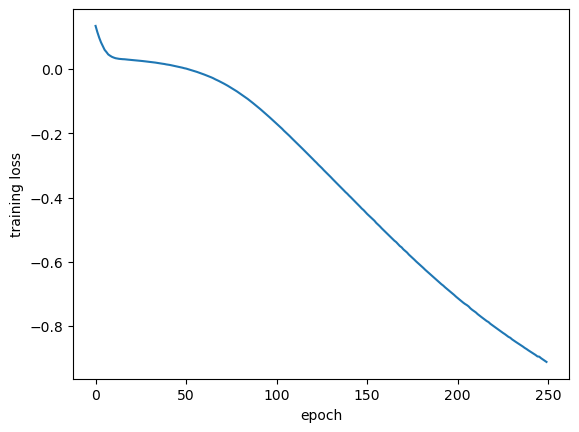
\includegraphics[height=130px]{../src_code/fig/p4/train_loss_t1}}
		\\ \hline
		t2 & 98.50\% & 97.78\% & \raisebox{-125px}{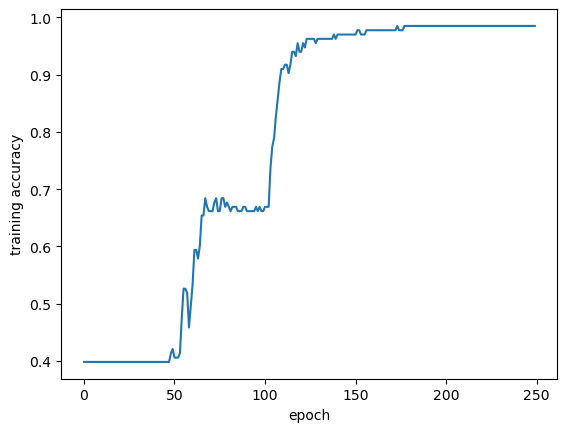
\includegraphics[height=130px]{../src_code/fig/p4/train_accu_t2}} & \raisebox{-125px}{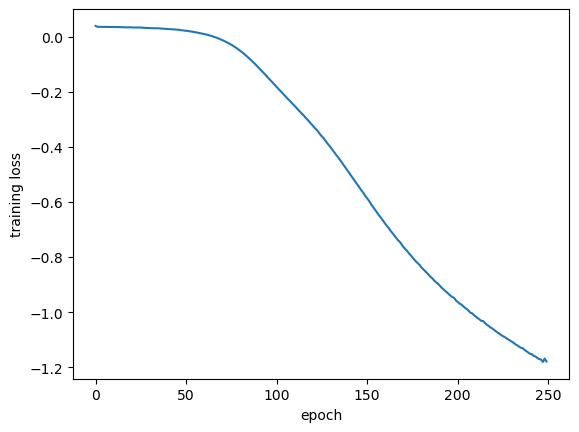
\includegraphics[height=130px]{../src_code/fig/p4/train_loss_t2}}
		\\ \hline
		t3 & 97.74\% & 88.89\% & \raisebox{-125px}{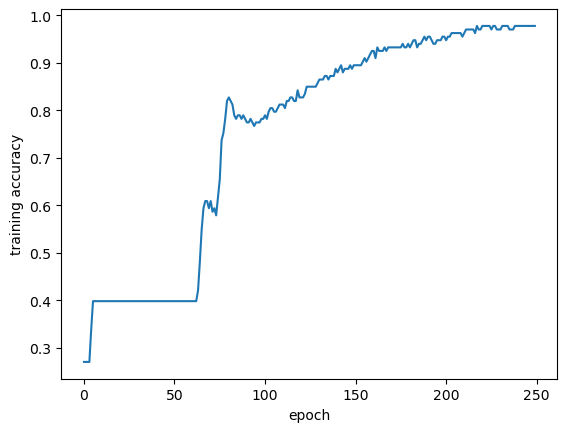
\includegraphics[height=130px]{../src_code/fig/p4/train_accu_t3}} & \raisebox{-125px}{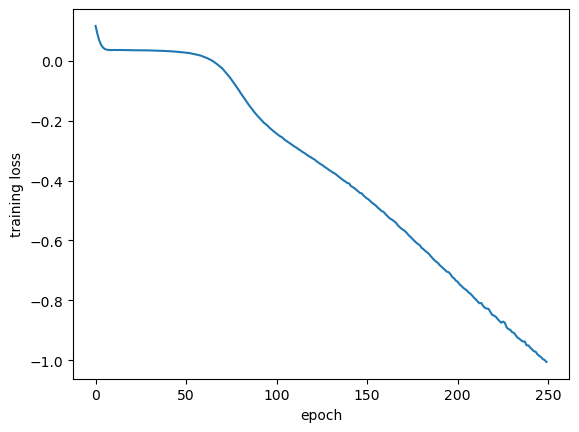
\includegraphics[height=130px]{../src_code/fig/p4/train_loss_t3}}
		\\ \hline
		t4 & 95.49\% & 91.11\% & \raisebox{-125px}{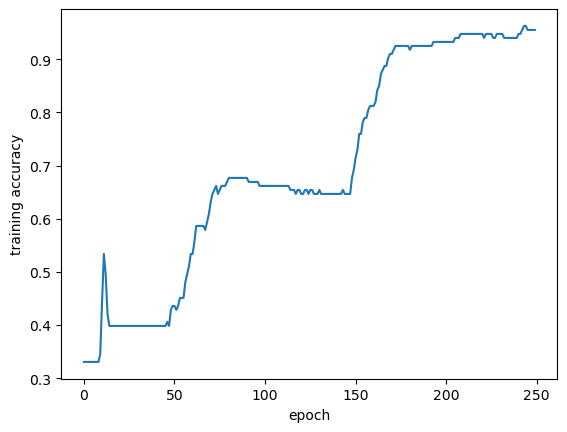
\includegraphics[height=130px]{../src_code/fig/p4/train_accu_t4}} & \raisebox{-125px}{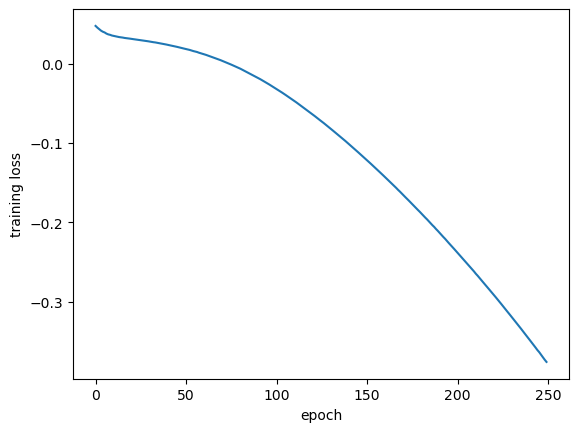
\includegraphics[height=130px]{../src_code/fig/p4/train_loss_t4}}
		\\ \hline
		t5 & 65.41\% & 64.44\% & \raisebox{-125px}{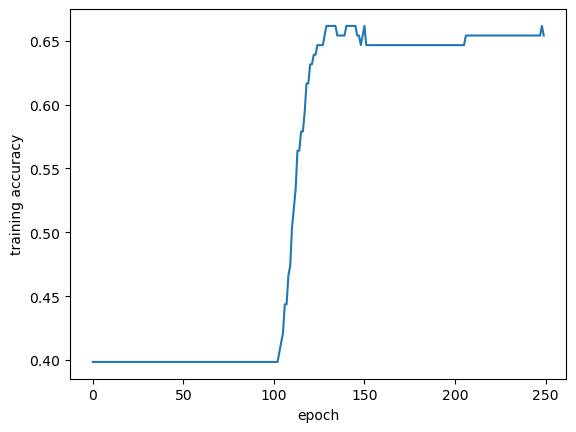
\includegraphics[height=130px]{../src_code/fig/p4/train_accu_t5}} & \raisebox{-125px}{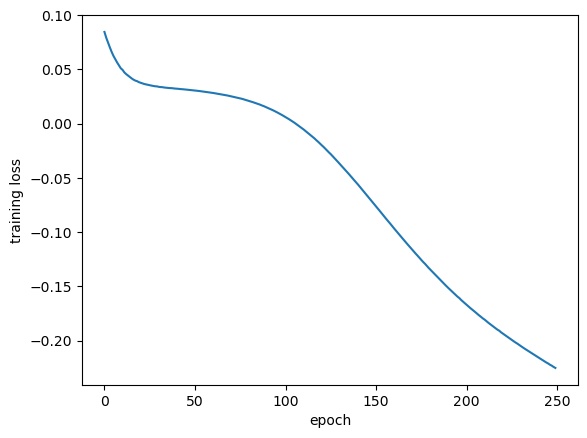
\includegraphics[height=130px]{../src_code/fig/p4/train_loss_t5}}
		\\ \hline
		t6 & 93.23\% & 88.89\% & \raisebox{-125px}{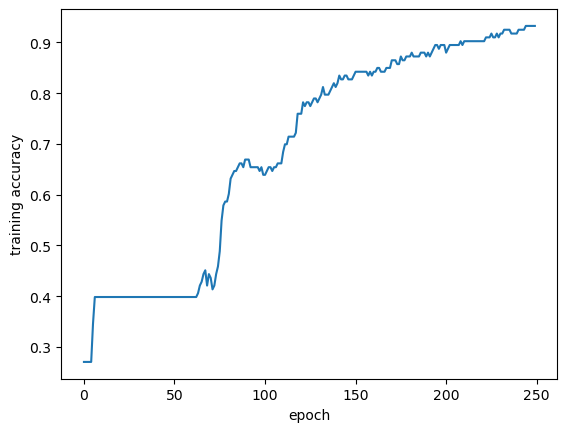
\includegraphics[height=130px]{../src_code/fig/p4/train_accu_t6}} & \raisebox{-125px}{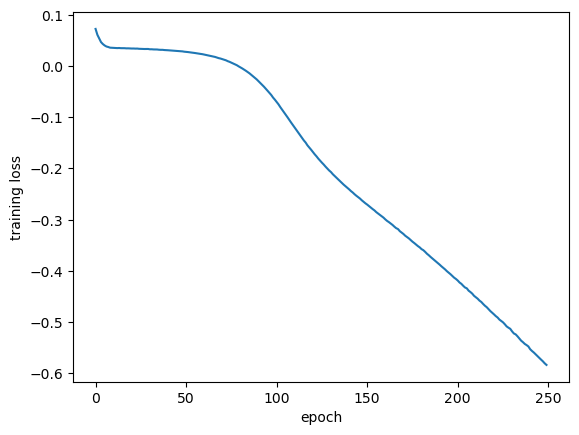
\includegraphics[height=130px]{../src_code/fig/p4/train_loss_t6}}
		\\ \hline
		\caption{Model Performance Summary Table} % needs to go inside longtable environment
		\label{table:train-result}
	\end{longtable}
%\end{table}

As \Cref{table:train-result} shown, and also seen in output \Cref{output:result} below, we may find the best performing model is the first model (\Cref{code:p4:best}) with 2 hidden layers and 10 and 20 neurons in the first and second layer respectively.

\lstinputlisting[language=python, caption=Best Model, label=code:p4:best, firstline=223, lastline=230]{../src_code/p4.py}	

\begin{lstlisting}[language=python, style=mystyle:output, label=output:result, caption=Python Output]
=== P4.1 ===
==== TEST [t1        ] ====
Train accuracy: 98.50 %
Test accuracy: 97.78 %
==== TEST [t2        ] ====
Train accuracy: 98.50 %
Test accuracy: 97.78 %
==== TEST [t3        ] ====
Train accuracy: 97.74 %
Test accuracy: 88.89 %
==== TEST [t4        ] ====
Train accuracy: 95.49 %
Test accuracy: 91.11 %
==== TEST [t5        ] ====
Train accuracy: 65.41 %
Test accuracy: 64.44 %
==== TEST [t6        ] ====
Train accuracy: 93.23 %
Test accuracy: 88.89 %
t1
{'mlp': <tensorflow.python.keras.engine.sequential.Sequential object at 0x7f8a36ff8a30>, 'max_epoch': 250, 'train_accuracy': 98.49624037742615, 'test_accuracy': 97.77777791023254}
\end{lstlisting}


\newpage
\subsection{Classification Test Result \label{sec:4:2}}
The classification result is as shown in \Cref{output:classification-result} below:
\begin{lstlisting}[language=python, style=mystyle:output, label=output:classification-result, caption=Test Result]
=== P4.2 ===
[13.72, 1.43, 2.5, 16.7, 108, 3.4, 3.67, 0.19, 2.04, 6.8, 0.89, 2.87, 1285]
Normalized: [[0.70789474 0.13636364 0.60962567 0.31443299 0.41304348 0.83448276
  0.70253165 0.11320755 0.51419558 0.47098976 0.33333333 0.58608059
  0.71825963]]
[test_a    ]: Predicted ranking array: [[0.97562927 0.02270135 0.00166926]], Classified as: 1
[12.04, 4.3, 2.38, 22, 80, 2.1, 1.75, 0.42, 1.35, 2.6, 0.79, 2.57, 580]
Normalized: [[0.26578947 0.70355731 0.54545455 0.58762887 0.10869565 0.3862069
  0.29746835 0.54716981 0.29652997 0.11262799 0.25203252 0.47619048
  0.21540656]]
[test_b    ]: Predicted ranking array: [[0.01448519 0.8093967  0.17611817]], Classified as: 2
[14.13, 4.1, 2.74, 24.5, 96, 2.05, 0.76, 0.56, 1.35, 9.2, 0.61, 1.6, 560]
Normalized: [[0.81578947 0.66403162 0.73796791 0.71649485 0.2826087  0.36896552
  0.08860759 0.81132075 0.29652997 0.67576792 0.10569106 0.12087912
  0.20114123]]
[test_c    ]: Predicted ranking array: [[0.0041227  0.02048865 0.9753887 ]], Classified as: 3
\end{lstlisting}

The \verb|`a'| dataset is classified as class 1, \verb|`b'| dataset is classified as class 2, \verb|`c'| dataset is classified as class 3.

%%%%%%%%%%%%%%%%%%%%%%%%%%%%%%%%%%%%%%%%%%%%%%%%%%%%%%%%%%%%%%%%%%%%%%%%%%%%%%%%
%% ************************************************************************** %%
%% *                      TODO [Remove For Final Copy!]                     * %%
%% ************************************************************************** %%
%%%%%%%%%%%%%%%%%%%%%%%%%%%%%%%%%%%%%%%%%%%%%%%%%%%%%%%%%%%%%%%%%%%%%%%%%%%%%%%%
%\printlistoftodos

%%%%%%%%%%%%%%%%%%%%%%%%%%%%%%%%%%%%%%%%%%%%%%%%%%%%%%%%%%%%%%%%%%%%%%%%%%%%%%%%
%% ************************************************************************** %%
%% *                                Glossary                                * %%
%% ************************************************************************** %%
%%%%%%%%%%%%%%%%%%%%%%%%%%%%%%%%%%%%%%%%%%%%%%%%%%%%%%%%%%%%%%%%%%%%%%%%%%%%%%%%
%\clearpage
%\printglossaries

%%%%%%%%%%%%%%%%%%%%%%%%%%%%%%%%%%%%%%%%%%%%%%%%%%%%%%%%%%%%%%%%%%%%%%%%%%%%%%%%
%% ************************************************************************** %%
%% *                               References                               * %%
%% ************************************************************************** %%
%%%%%%%%%%%%%%%%%%%%%%%%%%%%%%%%%%%%%%%%%%%%%%%%%%%%%%%%%%%%%%%%%%%%%%%%%%%%%%%%

% \printbibliography[heading=none]

%%%%%%%%%%%%%%%%%%%%%%%%%%%%%%%%%%%%%%%%%%%%%%%%%%%%%%%%%%%%%%%%%%%%%%%%%%%%%%%%
%% ************************************************************************** %%
%% *                               Appendices                               * %%
%% ************************************************************************** %%
%%%%%%%%%%%%%%%%%%%%%%%%%%%%%%%%%%%%%%%%%%%%%%%%%%%%%%%%%%%%%%%%%%%%%%%%%%%%%%%%
% appendices use section and subsection numbering
\newpage
\appendix
\begin{appendices}
% INPUT UR APPENDIX
\section{P1 - Code}
\lstinputlisting[language=python, caption=Perceptron and Adaline Implementation, label=code:p1]{../src_code/output_scripts/p1.py}

\section{P2 - Code}
\lstinputlisting[language=python, caption=Madaline Implementation, label=code:p2]{../src_code/p2.py}

\section{P3 - Code}
\lstinputlisting[language=python, caption=MLP k-Fold Hyperparameter Optimization, label=code:p3]{../src_code/p3.py}

\section{P4 - Code}
\lstinputlisting[language=python, caption=MLP Multi-class Classifier, label=code:p4]{../src_code/p4.py}


\end{appendices}

\end{document}


